\documentclass{article}
% \PassOptionsToPackage{numbers, square}{natbib}
\usepackage[final, nonatbib]{neurips_2019}
\usepackage[utf8]{inputenc} % allow utf-8 input
\usepackage[T1]{fontenc}    % use 8-bit T1 fonts
\usepackage[dvipsnames]{xcolor}
\definecolor{greenyellow}{rgb}{0.0, 0.0, 0.8}
\usepackage[colorlinks = true, urlcolor  = greenyellow, linkcolor = greenyellow, citecolor = greenyellow]{hyperref}       % hyperlinks
\usepackage{url}            % simple URL typesetting
\usepackage{booktabs}       % professional-quality tables
\usepackage{amsfonts}       % blackboard math symbols
\usepackage{nicefrac}       % compact symbols for 1/2, etc.
\usepackage{microtype}      % microtypography

\usepackage{graphicx}
\usepackage{float}
\usepackage{gensymb}
\usepackage{amsmath}
\usepackage{subfig}
\usepackage{bm}
\usepackage{wrapfig}

\usepackage{todonotes}

\renewcommand*{\sectionautorefname}{Section}
\renewcommand*{\subsectionautorefname}{Section}
\renewcommand*{\figureautorefname}{Figure}
\renewcommand*{\tableautorefname}{Table}

\renewcommand\thesubfigure{\alph{subfigure}}
\newcommand{\subfigureautorefname}{\figureautorefname}


% \usepackage[nottoc]{tocbibind}
% \usepackage[colorlinks=true, citecolor=blue, linkcolor=blue, urlcolor=blue]{hyperref}

\usepackage[numbers, square]{natbib}
% \setcitestyle{numbers, square}
\DeclareMathOperator*{\argmax}{arg\,max}

\title{Reproducibility Challenge -- Generative Modeling by Estimating Gradients of the Data Distribution}

\author{%
  Antonio Matosevic \\
  \texttt{matose@kth.se} \\
  \And
  Eliisabet Hein \\
  \texttt{elihei@kth.se} \\
  \And
  Francesco Nuzzo \\
  \texttt{fnuzzo@kth.se} \\
}

\begin{document}

\maketitle

% \begin{abstract}
%     In this project we attempt to reproduce results from the paper \textit{Generative Modeling by Estimating Gradients of the Data Distribution} by \citet{ncsn-paper}. The authors propose a novel generative framework based solely on gradients of data density estimated by a neural network. Once the model is trained, sampling can be performed with annealed Langevin dynamics. While we managed to reproduce the experiments qualitatively, we failed to achieve comparable results for Inception and FID scores for CIFAR-10. We further extended the original work in various directions (computing and analysing FID and IS also for CelebA, investigation of the sampling hyperparameters $\epsilon$ and $T$, linear instead of geometric annealing schedule for noise levels, and different network architecture).
% \end{abstract}


\section{Introduction}
Recent popular deep generative models can roughly be categorised as either adversarial (GANs) or likelihood-based (VAEs, autoregressive, flow-based). While the former often suffer from unstable training, the latter require a particular architecture or a surrogate loss.
\citet{ncsn-paper} introduce a novel method based on estimating the gradients of data log-density with respect to the input data (i.e. \textit{score}).

Subsequently, during sampling, an initial random point is moved to a high-density region by using the estimated gradient. In this report, we investigate the reproducibility of %experiments in 
\cite{ncsn-paper}. For this purpose, we briefly introduce the method (\autoref{sec:method}), present the implementation details and comment on the reproducibility (\autoref{sec:implementation}), provide the results of toy (\autoref{sec:repr-of-toy}) and main (\autoref{sec:main-exp}) experiments, as well as propose and test extensions to the original paper (\autoref{sec:additional}).


\section{Method}
\label{sec:method}

\paragraph{Score estimation} \label{score_est} One major component of the proposed approach is direct estimation of the score $\nabla_{\mathbf{x}} \log p(\mathbf{x})$ using a neural network $s_{\bm{\theta}}(\mathbf{x})$, thus circumventing estimation of the data density $p(\mathbf{x})$. To this end, the theoretical objective $\frac{1}{2}\mathbb{E}_p\left[ || s_{\bm{\theta}}(\mathbf{x}) - \nabla_{\mathbf{x}} \log p(\mathbf{x})  ||^2_2 \right]$ can be reformulated in different ways to get two different loss functions, %for $s_{\bm{\theta}}$
sliced score matching (SSM) \citep{ssm} and denoising score matching (DSM) \citep{dsm}. SSM uses projections on random vectors $\mathbf{v} \sim p(\mathbf{v}) = \mathcal{N}(\mathbf{0}, \mathbf{I})$ and is given as
\begin{equation}
\mathbb{E}_{p_{\mathbf{v}}}\mathbb{E}_{p(\mathbf{x})}\left[ \mathbf{v}^{\text{T}}\nabla_{\mathbf{x}}s_{\bm{\theta}}(\mathbf{x})\mathbf{v} + \frac{1}{2}||s_{\bm{\theta}}(\mathbf{x}))||^2_2 \right].
\end{equation}
While the SSM loss is exact, it is slow to compute, so often in practice DSM loss is used instead. DSM loss estimates the score of density for perturbed data $ \mathbf{\tilde x}$ and is given as
\begin{equation}
\frac{1}{2} \mathbb{E}_{q_\sigma ( \mathbf{ \tilde x} | \mathbf{x}) p(\mathbf{x})} \left[ || s_{\bm{\theta}}( \mathbf{ \tilde x}) - \nabla_{\mathbf{\tilde x}} \log q_\sigma( \mathbf{ \tilde x} | \mathbf{x})  ||^2_2  \right],
\end{equation}
where $q_\sigma( \mathbf{ \tilde x} | \mathbf{x}) = \mathcal{N}(\mathbf{x}, \sigma^2\mathbf{I})$ in \cite{ncsn-paper}. Intuitively, a perturbed $\mathbf{\tilde x}$ should move us towards the original $\mathbf{x}$. In fact, it holds that $s^*_{\bm{\theta}}(\mathbf{x})  = \nabla_{\mathbf{x}} \log q_{\sigma} (\mathbf{x}) \approx \nabla_{\mathbf{x}} \log p(\mathbf{x})$ for $\sigma$ small enough so that $q_{\sigma}(\mathbf{x}) \approx p(\mathbf{x})$.

\paragraph{Sampling}\label{sampling} Using scores for generative modelling relies on sampling with Langevin dynamics. Namely, given a step size $\epsilon > 0$ and an initial value $\mathbf{\tilde x}_0$ we can, using only the score, compute $\mathbf{\tilde x}_t = \mathbf{\tilde x}_{t-1} + \frac{\epsilon}{2}\nabla_{\mathbf{x}}s^*_{\bm{\theta}}(\mathbf{\tilde x}_{t-1})  + \sqrt{\epsilon}\ \mathbf{z}_t$, where $\mathbf{z}_t \sim \mathcal{N}(\mathbf{0}, \mathbf{I})$, for $T$ steps. It has been shown that under some regularity conditions $\mathbf{\tilde x}_T$ is an exact sample from $p(\mathbf{x})$ as $T \to \infty$ and $\epsilon \to 0$ \cite{Welling:2011:BLV:3104482.3104568}.

\vspace{1mm}

Unfortunately, direct implementation of the proposed framework usually suffers from two major issues, which the authors attribute to the manifold hypothesis and low-density regions of $p(\mathbf{x})$. 

\paragraph{Manifold hypothesis} For most natural images, the manifold hypothesis states that the intrinsic dimensionality of $\mathbf{x}$ has a support in $\mathbb{R}^M \subset \mathbb{R}^D$, where $M \ll D$. As a consequence, a score (gradient) taken in $\mathbb{R}^D$ is not going to be defined in $\mathbb{R}^M$. We will demonstrate the effects of this on training the score network by replicating a toy example from \cite{ncsn-paper} (\autoref{sec:repr-of-toy}).

\paragraph{Low-density regions} A negative effect of low-density regions concerns both score estimation and sampling. 
Firstly, the number of samples from low-density regions of $p(\mathbf{x})$ is not sufficient to accurately estimate the loss (i.e. scores) during training. Following \cite{ncsn-paper}, we visualise this by comparing analytic and estimated scores of a mixture of two Gaussians with near-zero density regions between the modes (\autoref{sec:repr-of-toy}).
Regarding sampling, Langevin dynamics require an infeasible number of iterations in traversing these regions to obtain good mixing. We successfully reproduce an experiment showing this on the same GMM (\autoref{sec:repr-of-toy}).

\paragraph{Proposed solutions}
Firstly, to remedy the negative implications of the manifold hypothesis, \citet{ncsn-paper} suggest adding Gaussian noise to data. Since the noise is defined in $\mathbb{R}^D$, this results in gradients being defined everywhere. Secondly, the authors observe that adding large noise also helps to fill in the low-density regions, hence improving the score estimation. Thirdly, while large noise helps during the training, it is not favourable for sampling. To address this issue, they propose obtaining a sample by iteratively generating from distributions of perturbed data $\{q_{\sigma_i}\}_{i=1}^L$ parameterised by a decreasing geometric sequence $\{\sigma_i\}_{i=1}^L$ of noise levels. This way one utilises the benefits of large noise to avoid low-density regions, but also gradually transitions to small noise where the perturbed data distribution is indistinguishable from $p(\mathbf{x})$. In practice, this requires only a small modification to Langevin dynamics described in \autoref{sampling} by embedding it into iterations over noise levels\footnote{Note that $\mathbf{x}_{\sigma_i} \sim q_{\sigma_i}$ is used to initialise sampling from $q_{\sigma_{i+1}}$. The intuition is that $\mathbf{x}_{\sigma_i}$ comes from a high-density region of $q_{\sigma_i}$ and since $q_{\sigma_i}$ and $q_{\sigma_{i+1}}$ are similar, $\mathbf{x}_{\sigma_i}$ is also in a high-density region of $q_{\sigma_{i+1}}$.} and multiplying $\epsilon$ by a factor of ${\sigma_i}^2/{\sigma_L}^2$. To employ this procedure, a single score network is trained with the total loss $\mathcal{L}(\bm{\theta}; \{\sigma_l\}_{l=1}^L) = \frac{1}{L}\sum_{l=1}^L \lambda(\sigma_l) \ell (\bm{\theta}; \sigma_i)$, where $\ell(\cdot)$ is a DSM loss\footnote{Well-motivated since we are now estimating the score of perturbed data.}, and $\lambda(\cdot)$ a parameter regulating that none of the individual loss terms dominates ($\sigma_i^2$ in \cite{ncsn-paper}).



\section{Implementation}
\label{sec:implementation}

All implementation was done in Python using TensorFlow 2.0, and the models were trained using P100 and V100 GPUs on the Google Cloud Platform. The original code by the authors was provided in PyTorch. To our knowledge, this is the first time this method has been ported to a new framework. Our code is available on GitHub at \url{https://www.github.com/Xemnas0/NCSN-TF2.0}.

\subsection{Data pipeline}
\label{sec:data-pipeline}

Since the datasets used (MNIST, CIFAR-10 and CelebA) are standard, we obtained them through the TensorFlow datasets API%\footnote{\url{https://www.tensorflow.org/datasets}}
. We used the standard training split for each dataset (60,000 samples for MNIST and CIFAR-10, and 162,770 samples for CelebA). We applied preprocessing to the data following \cite{ncsn-paper}. For CelebA, we extracted a $140\times140$ centre crop from the image and then resized to $32\times32$. Since the original paper does not specify which interpolation method to use for resizing, we used the default in TensorFlow (bilinear). For all the datasets, we scaled the values from [0, 255] to [0, 1] by dividing each pixel value by 255. Finally, for CIFAR-10 and CelebA, we also flipped each image along the vertical axis with 50\% probability each time a batch was loaded. The data was shuffled at the beginning of every epoch with a buffer size of 10,000 and then split into batches. After consulting with the published code, we noted that instead of using the default, the authors create a randomly sampled training split for MNIST and CelebA, and shuffle the whole dataset each epoch, but since our buffer is reasonably large, we do not consider these differences significant.

\subsection{Network architecture}
\label{sec:architecture}
An important aspect of the method is choice of the score network. The authors used three architectures (MLP and ResNet for toy experiments and RefineNet for the main experiment). As in \cite{ncsn-paper}, all models were trained with Adam optimizer with learning rate 0.001% and default parameters ($\beta_1=0.9$, $\beta_2=0.999$)
. For all experiments, batch size was 128. For ResNet and RefineNet, we used 64 filters for MNIST and 128 for CIFAR-10 and CelebA.

\paragraph{MLP} For the results in \autoref{fig:est-grad}, following \cite{ncsn-paper}, we use a three-layer MLP with 128 units per layer with softplus activation. While this was not specified by the authors, we do not apply activations to the outputs in any architecture, to keep the scores unnormalized and unbounded.

\paragraph{ResNet} For the results in \autoref{fig:toy1}, we use a ResNet encoder-decoder network as in \cite{ncsn-paper}. The encoder consists of 5 pre-activation residual blocks with 32, 64, 64, 128, 128 filters in each layer respectively, mirrored in the decoder. Downsampling/upsampling is performed at the end of the 2nd and 4th residual blocks in the encoder and decoder respectively. Activation function is ELU. For the details that were not specified in the paper, we made the following assumptions:
\begin{itemize} 
    \item  Convolutions (encoder) or transposed convolutions (decoder) are of size $3\times 3$.
    \item Resizing is performed with (transposed) convolutions of stride 2.
    \item Normalisation is done over batches and only within the residual blocks.
    \item For changing the number of filters within a skip connection, we use 1$\times$1 convolutions.
\end{itemize}



\paragraph{RefineNet}
The architecture in \cite{ncsn-paper} follows a 4-cascades RefineNet \citep{refinenet} adjusted to account for different noise levels. In short, the RefineNet is a variant of U-Net with residual blocks, where the upwards cascade consists of RefineBlocks, each of which in turn consists of three components: \textit{residual convolutional units} (RCU), \textit{multi-resolution fusion} (MRF) and \textit{chained residual pooling} (CRP). Since the architecture is complex, for brevity we refer to \cite{refinenet} for the exact details and to \cite{ncsn-paper} for the modifications made to it. From a reproducibility standpoint, we found the wording in the architecture description ambiguous; we contacted the authors for clarifications on certain details and were referred to the official code\footnote{\url{https://github.com/ermongroup/ncsn}}. Since the aim of this challenge was to test the reproducibility of the paper, we tried to rely only on that as much as possible, and checked the published code only when we could not make a justified assumption based on standard practice. Specifically, the aspects that were not clear from the paper, and the assumptions we made accordingly, were as follows:

\begin{itemize}
    \item \textbf{Number of ResNet blocks}: In \cite{refinenet}, the downward cascade (inputs to the RefineBlocks) are obtained from %different stages of 
    a ResNet pre-trained on ImageNet. In \cite{ncsn-paper} an unspecified number of pre-activation ResNet blocks per cascade was trained from scratch instead. Referring to the code, we found 2 such blocks were used. In correspondence the authors said there was no specific reason for this number and that it should be robust to different choices, so we used only 1 due to computational limitations. 
    \item \textbf{Dilated convolution}: The authors replace regular convolutions in the ResNet blocks with dilated convolutions. While the paper claims to increase the dilation by a factor of two in each cascade (which we interpreted as dilation rates 1, 2, 4, 8 corresponding to the four cascades), this would result in extremely large dilations relative to the size of the image in the lowest cascade. In the code, the authors use dilation rates 1, 1, 2, 4, while we decided to apply 1, 2, 2, 4 as a compromise between what is claimed in the paper -- that dilated convolutions are not used only in the first cascade -- and the aforementioned issue. %We use the dilation rates used in the authors' code, 1, 2, 2, 4 in the four cascades respectively.
    \item \textbf{Downsampling}: It was not specified how and where downsampling was done in the downward cascade, so we referred to the code and found that it was performed by $2\times 2$ average pooling with stride 2, and only after the first cascade. We would like to emphasize that the phrasing in the original paper is ambiguous in this regard, giving the impression that dilated convolutions are used to perform downsampling, when in reality this was not the case.
    \item \textbf{Filters}: Based on the authors' code, we used 3$\times$3  convolutions at the beginning and the end of the architecture to move between input channels and number of filters. 
    
    Following the description in the original paper, we also doubled the number of filters in all layers corresponding to the 2nd, 3rd and 4th cascades, and in the residual blocks where the number of filters is doubled, we added another 1$\times$1 convolution to also double the filters in the skip connection, as is standard practice. However, we later found that this differs slightly from how the authors' implementation -- they increase the number of filters in the final convolution of the 1st cascade, whereas we do it in the first convolution of the 2nd cascade, and they use 3$\times$3 convolutions to increase the number of filters in the skip connections. We further noticed that the authors have 3$\times$3 convolutions in the skip connections of the first residual block of each cascade even when the number of filters does not change.
    %\item Since not given, we chose kernel size 1 when changing the number of filters and 3 otherwise.
    \item %The authors introduce instance normalisation conditioned on noise and place this before every convolution in the network, except the first one as it is not common practice to normalise the raw input.
    \textbf{Initialisation of normalisation parameters}: Since these values were not specified, we initialized the $\alpha$ and $\gamma$ parameters for conditional instance normalisation to ones (instead on $\mathcal{N}(1, 0.02)$ as in the code), and $\beta$ to zeros, as is common practice for batch normalisation.
\end{itemize}




\subsection{Evaluation}
\label{sec:eval}

Due to limited computational resources we save checkpoints during training every 10,000 iterations instead of every 5,000 as in \cite{ncsn-paper}. We choose the best model for CIFAR-10 and CelebA by computing the FID on 1000 samples generated from each checkpoint. For MNIST we used the final model as in \cite{ncsn-paper}. The reported Inception score and FID were computed on 50,000 samples from the best model.


\section{Reproduction of toy experiments}
\label{sec:repr-of-toy}


The first experiment tests whether perturbing the data with small Gaussian noise $\mathcal{N}(0, 0.0001)$ addresses the problem with the manifold hypothesis and facilitates learning. %(implying that the score was not defined before adding noise). %, implicitly meaning the score is defined where it otherwise would not be because of the manifold hypothesis. 
As in \citep{ncsn-paper}, we trained a ResNet encoder-decoder (\autoref{sec:architecture}) on CIFAR-10 with SSM loss for 50,000 iterations (\autoref{fig:toy1}). While we do not get exactly the same magnitude or behaviour of the loss curves as in \cite{ncsn-paper}, we can confirm that the model only converges with perturbed data.% We have included the loss curves in . 

\begin{figure}[h]
  \centering
  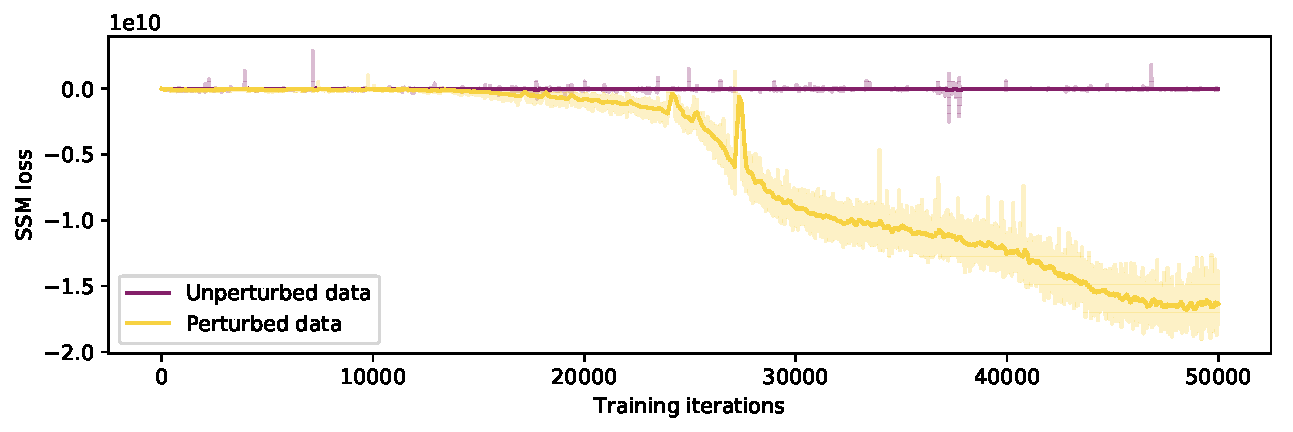
\includegraphics[width=0.83\linewidth]{figures/toy/loss_toy.pdf}
     \caption{Loss curves for score networks trained on
     CIFAR-10 before and after perturbing the data.}
     \label{fig:toy1}
     \vspace{-3mm}
\end{figure}

In the second experiment we compared analytically computed scores (\autoref{fig:anal-grad}) with those estimated by an MLP (\autoref{sec:architecture}) trained with SSM loss for 10,000 iterations (\autoref{fig:est-grad}) for a GMM with $p(\mathbf{x}) = 0.2\ \mathcal{N}\left((-5, -5), \mathbf{I}\right) + 0.8\ \mathcal{N}\left((5, 5), \mathbf{I}\right)$ with near-zero density between the components. The plots look similar to those from the original paper. We can see that scores estimation is accurate in high-density regions around the modes, but fails in low-density ones, as expected.
% \vspace{-2mm}

\begin{figure}[H]
  \centering
     \subfloat[Density of the data]{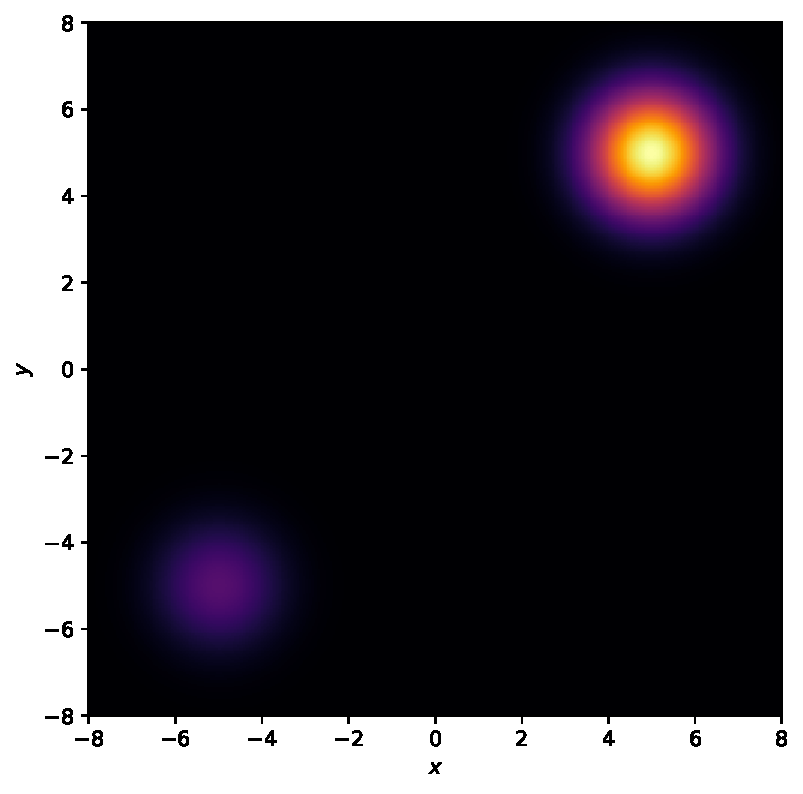
\includegraphics[scale=0.26]{figures/toy/density.pdf}\label{fig:density}}
     \subfloat[True score]{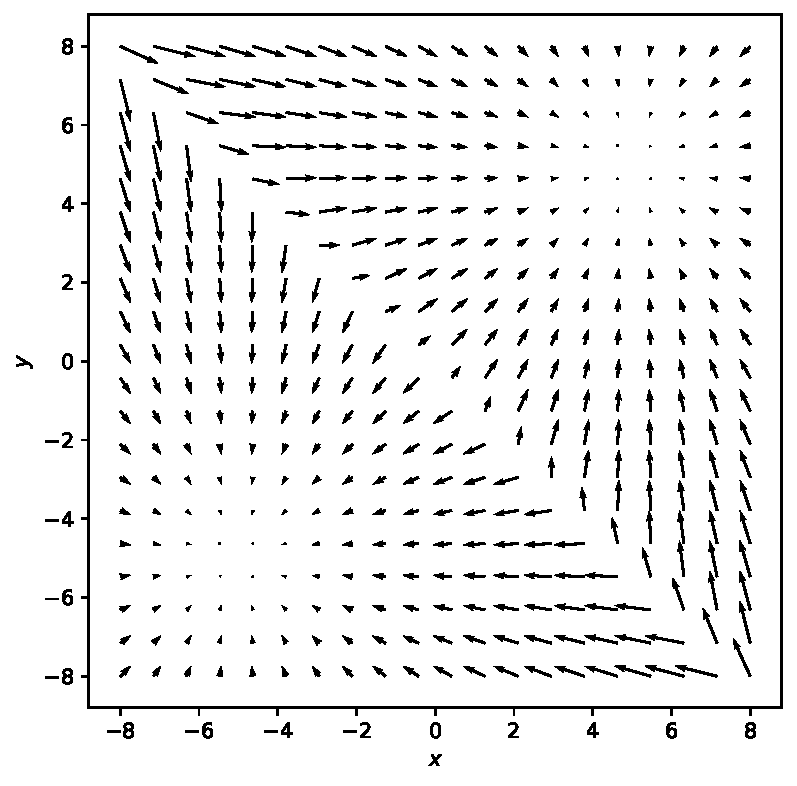
\includegraphics[scale=0.26]{figures/toy/grad_analytic.pdf}\label{fig:anal-grad}}
     \subfloat[Estimated score]{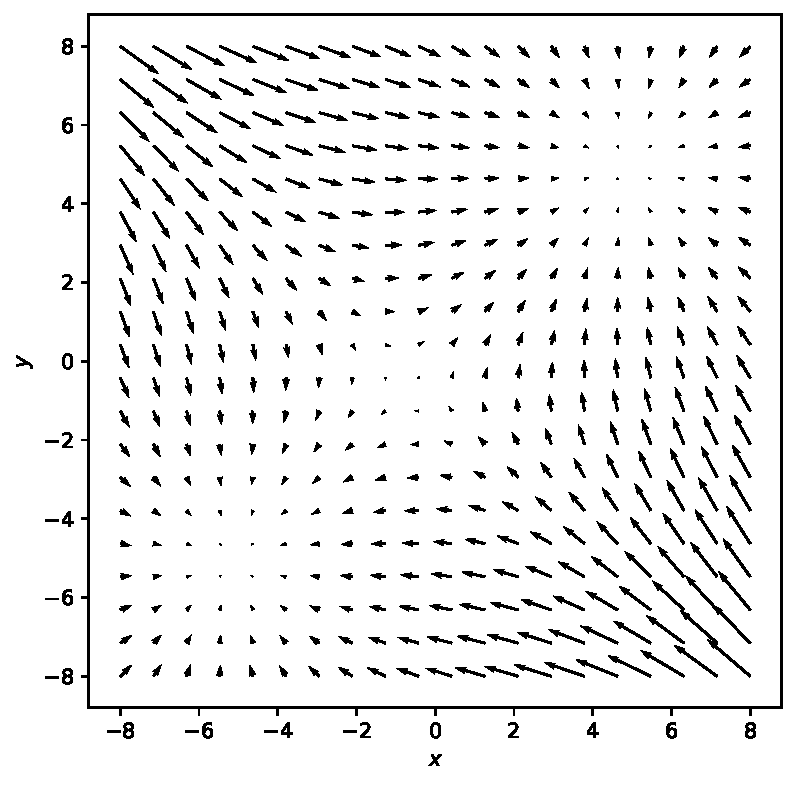
\includegraphics[scale=0.26]{figures/toy/grad-est.pdf}\label{fig:est-grad}}
     \caption{Effect of low-density regions on score estimation.}
     \label{fig:toy2}
     \vspace{-3mm}
\end{figure}

% \subsection{Sampling with Langevin dynamics}
% \label{sec:toy-sampling}

Finally, we attempted to reproduce Figure 3 from the original paper to show the effect of low-density regions on sampling using Langevin dynamics with and without annealing from the GMM from the previous experiment. Here we used the true scores computed analytically. \citet{ncsn-paper} claim that they used a geometric sequence of 10 noise levels $\sigma$ between 10 to 0.1, $T=100$ and $\epsilon=0.1$. However, with this setup, we failed to reproduce the plot (no samples were obtained because of numerical overflow).\footnote{We also confirmed that running the authors' code with these parameters gave the same results.} When consulting with the authors' code, we found that unlike what was reported in \citep{ncsn-paper}, a geometric sequence between 20 and $e^{0.1}$ was used. With these values, we indeed obtained a very similar plot (\autoref{fig:samp-anneal}) to what was reported in the paper.
%\vspace{-2mm}

\begin{figure}[h!]
  \centering
     \subfloat[Exact samples]{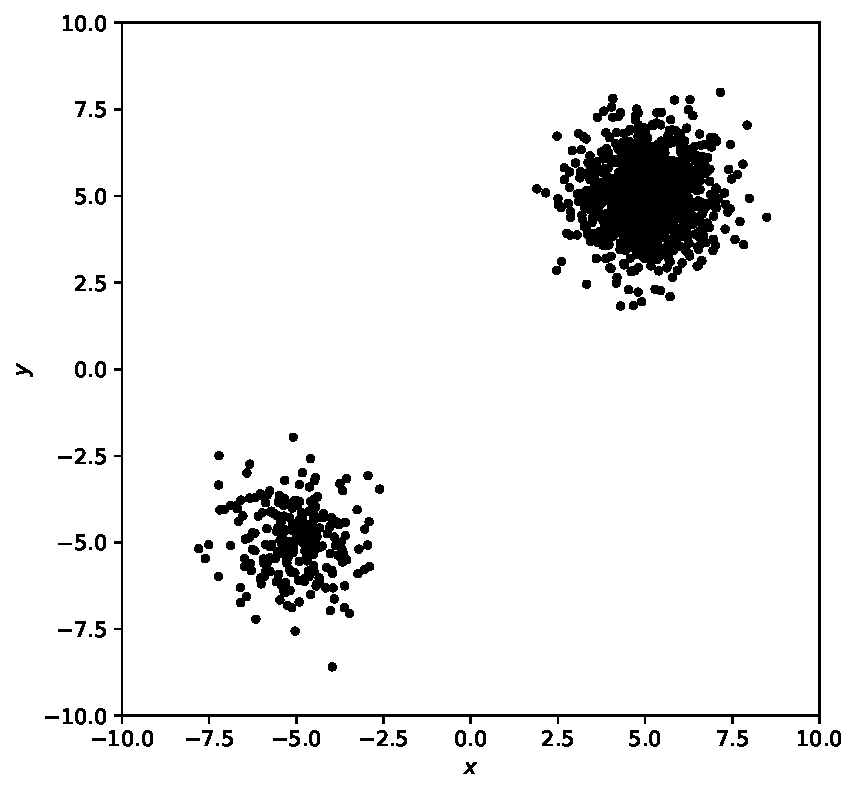
\includegraphics[scale=0.26]{figures/toy/real_samples.pdf}\label{fig:samp}}
     \subfloat[Samples without annealing]{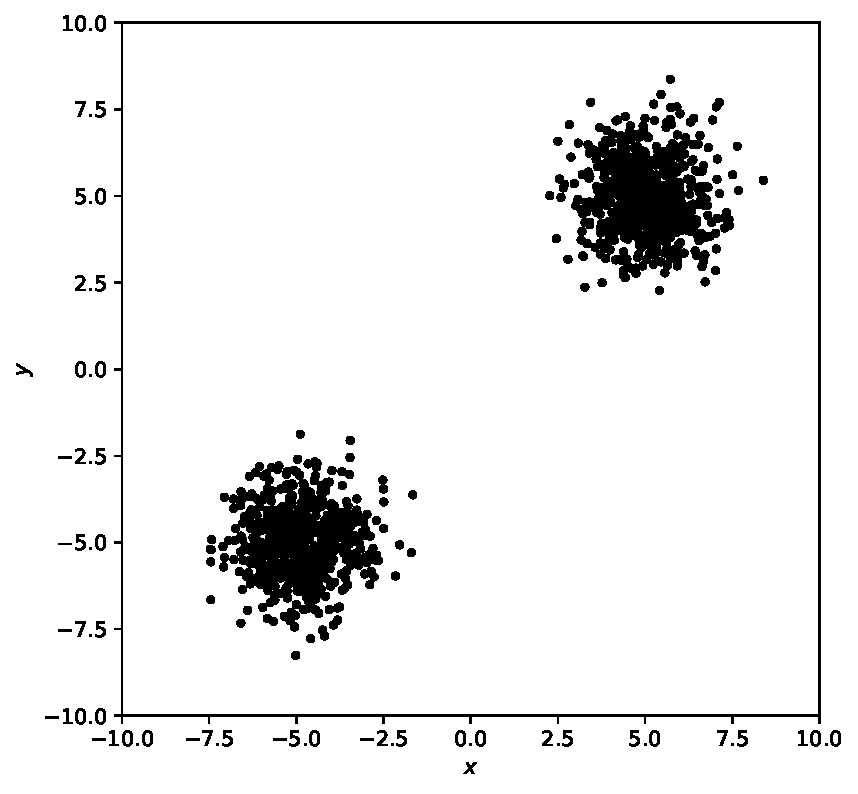
\includegraphics[scale=0.26]{figures/toy/samples_langevin.pdf}\label{fig:samp-langevin}}
     \subfloat[Samples with annealing]{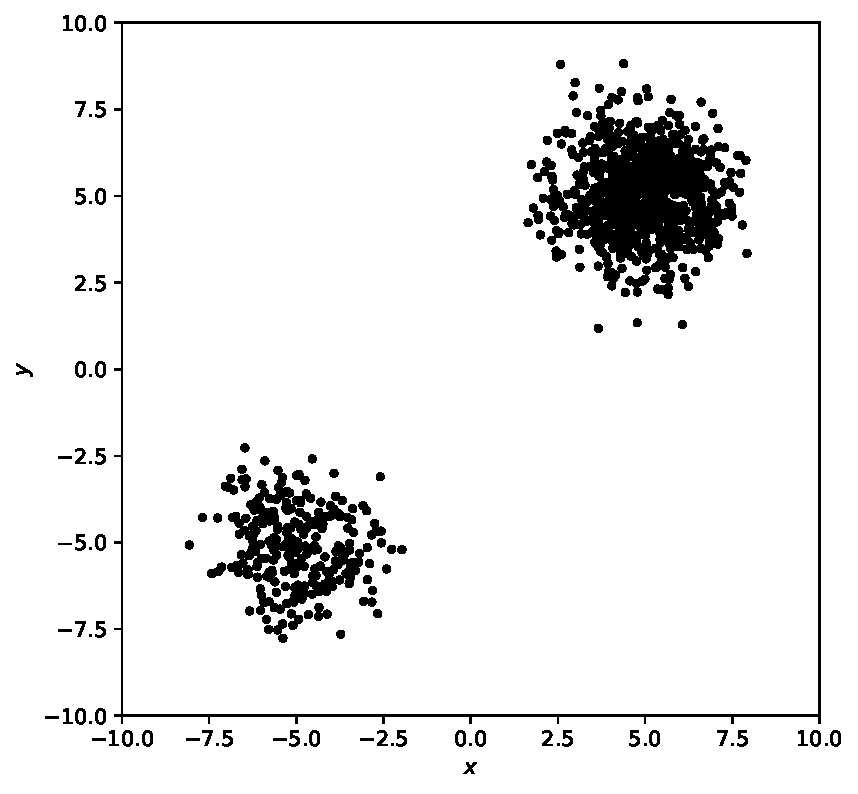
\includegraphics[scale=0.26]{figures/toy/samples_annealed_langevin.pdf}\label{fig:samp-anneal}}
     \caption{Effect of low-density regions on sampling with Langevin dynamics.}
     \label{fig:toy3}
    %  \vspace{-2mm}
\end{figure}

We reason that the reported hyperparameters fail due to step size $\epsilon(\sigma_1 / \sigma_L)^2$, which becomes relatively large when $\epsilon$ and $\sigma_1$ are large or $\sigma_L$ is small. The authors avoid the issue by increasing $\sigma_L$.\footnote{This could be by mistake as the logarithm is applied to $\sigma_1$ but not to $\sigma_L$ when constructing the sequence.} However, this goes against the idea of annealed Langevin dynamics, which is to converge to a distribution which is almost indistinguishable from the true one (i.e. having small $\sigma_L$ is desirable). Therefore we decided to experiment with decreasing $\epsilon$ instead. We include the results in \autoref{fig:eps} in the Appendix. Even with extensive fine-tuning of $\epsilon$ we did not manage to get visually satisfying results, so it is clear that the algorithm is very sensitive to the choice of this hyperparameter. We suggest a goodness-of-fit or a comparison of likelihoods as the future work to quantitatively assess the similarity of distributions.


\section{Reproduction of main experiment}
\label{sec:main-exp}

In this section, we present our reproduction of the main experiments from \citep{ncsn-paper}, which consist of training RefineNet models (\autoref{sec:architecture}) on MNIST, CIFAR-10 and CelebA datasets and performing sampling and inpainting with the best models. Following \cite{ncsn-paper}, the baseline was trained without annealing, conditioned on only one noise level ($\sigma=0.01$), while the final model was conditioned on a geometric sequence $\{\sigma_i\}_{i = 1}^{10}$ from 1 to 0.01. All models were trained for 200,000 iterations. 

\subsection{Image generation}

\begin{wrapfigure}{h!}{0.39\textwidth}
    \centering
    \vspace{-2mm}
    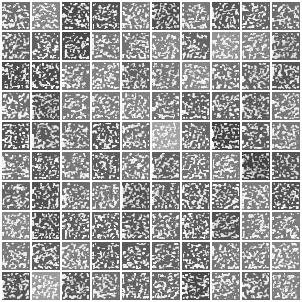
\includegraphics[scale=0.38]{figures/samples/baseline.png}
    \caption{Samples from the baseline.}
    \label{fig:baseline}
    \vspace{-2mm}
\end{wrapfigure}

\paragraph{One noise level}
The samples generated from the baseline model trained on MNIST are given in \autoref{fig:baseline}. Following \cite{ncsn-paper}, we used $T=1000$ and $\epsilon=2 \cdot 10^{-5}$ for sampling. As we can see, the model fails to generate correct samples, which is in agreement with the original results, even for a simple dataset such as MNIST. Due to limited computational resources, we omit training the baseline for CIFAR-10 and CelebA, and focus instead on additional experiments. Overall, we consider this choice of baseline redundant, as the importance of multiple noise levels has already been showcased on the toy example (\autoref{sec:repr-of-toy}). In our opinion, a more informative baseline would be a simplified network architecture or simpler annealing schedule; we will investigate this in \autoref{sec:additional}.

\paragraph{Multiple noise levels} We now present our results from replicating the main experiments with models trained with a geometric sequence $\{\sigma_i\}_{i=1}^{10}$, to showcase that this approach yields reasonable samples of real data. The loss curves are given in \autoref{fig:losses} in the Appendix. We chose the best model from checkpoints as explained in \autoref{sec:eval}. The samples obtained from this model with $T=100$ and $\epsilon=2 \cdot 10^{-5}$ and intermediate samples from each $q_{\sigma_i}$ are shown in \autoref{fig:samp}. Additional samples are provided in the Appendix. The best model for CIFAR-10 was found at 120k iterations and for CelebA at 30k. The Inception score and FID computed from 50k samples from the final model for CIFAR-10 were \bm{$6.5 \pm 0.118$} and \bm{$33.0$}, and for CelebA \bm{$3.4 \pm 0.0395$} and \bm{$81.5$}.

\begin{figure}[h!]
  \centering
     \subfloat[MNIST samples]{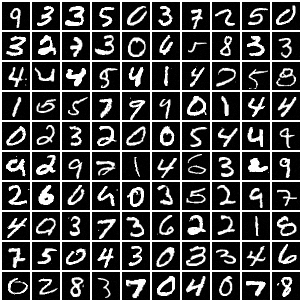
\includegraphics[width=0.31\linewidth]{figures/samples/mnist_samples.png}\label{fig:mnist-samp}}\hspace{2mm}
     \subfloat[CIFAR-10 samples]{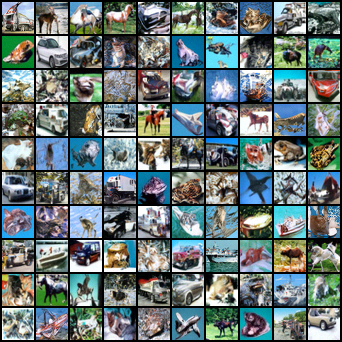
\includegraphics[width=0.31\linewidth]{figures/samples/refinenet128_cifar10_L10_step120000.png}\label{fig:cifar10-samp}}\hspace{2mm}
     \subfloat[CelebA samples]{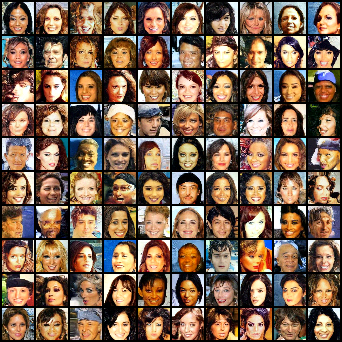
\includegraphics[width=0.31\linewidth]{figures/samples/celeba_samples.png}\label{fig:celeba-samp}} \\
     \subfloat[MNIST intermediate]{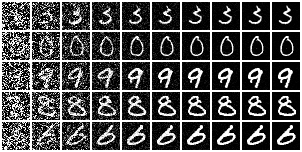
\includegraphics[width=0.31\linewidth]{figures/samples/refinenet64_mnist_L10_step200000_intermediate.png}\label{fig:mnist-intermediate}}\hspace{2mm}
     \subfloat[CIFAR-10 intermediate]{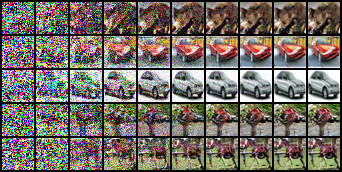
\includegraphics[width=0.31\linewidth]{figures/samples/refinenet128_cifar10_L10_step120000_intermediate.png}\label{fig:cifar10-intermediate}}\hspace{2mm}
     \subfloat[CelebA intermediate]{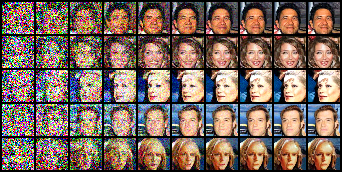
\includegraphics[width=0.31\linewidth]{figures/samples/refinenet128_celeb_a_L10_step30000_intermediate.png}\label{fig:celeba-intermediate}}
     
     \caption{Uncurated samples generated from trained models for MNIST, CIFAR-10 and CelebA datasets with annealed Langevin dynamics (a-c) and intermediate steps during sampling process (d-f).}
     \label{fig:samples}
     \vspace{-3mm}
\end{figure}

As we can see, while the samples are qualitatively good, our Inception and FID scores for CIFAR-10 are noticeably worse than those reported in the paper (8.87$\pm$.12 and 25.32, respectively). A possible reason could be the high variability in the FID score when choosing the best model as described in \autoref{sec:eval}; we show that the FID score fluctuates for checkpoints for both CIFAR-10 and CelebA in \autoref{fig:fid} in the Appendix. We believe using more samples at each checkpoint (the standard for FID is a minimum of 2048, while here we only used 1000 as per \cite{ncsn-paper}) would yield a more reliable metric, but this comes at the cost of more expensive computations. There could also be some differences in the architecture that were missed in the implementation.\footnote{We initially considered the number of residual blocks, but with 2 blocks the results did not improve.} As an extension to the original paper, we also computed FID and IS for CelebA. While cropping and resizing means that results are not directly comparable to results from literature, we can see that our achieved results are significantly worse -- the current reported state of the art FID score for $64 \times 64$ CelebA is $4.00$ \cite{DBLP:journals/corr/abs-1904-00284}, while we obtained $81.5$. Perhaps an interesting observation is that there are more female than male faces generated, which also reflects the ratio of these in the training data. In the interest of reproducability, we also report the time cost of training and sampling for each dataset in \autoref{tab:times} in the Appendix.

% \subsection{Nearest neighbours}
Following \cite{ncsn-paper}, we find $k$ nearest neighbours for a set of generated samples from the training data with respect to $l_2$ distance. Results are shown in \autoref{fig:nn}, and more extensive examples in \autoref{fig:nn-large} in the Appendix. As we can see, the network has not memorised exact training images, but still preserves some high-level features from the training set such as colour, shape, style, orientation etc.\footnote{\textbf{Disclaimer}: We implemented this before the authors added nearest-neighbour calculations to their work on 29th Oct 2019, which additionally measures distance based on activations from the Inception network.}\vspace{-4mm}

\begin{figure}[h!]
  \centering
     \subfloat[MNIST]{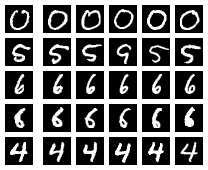
\includegraphics[width=0.28\linewidth]{figures/samples/refinenet64_mnist_L10_step200000_5nearest.png}\label{fig:mnist-nn}}\hspace{3mm}
     \subfloat[CIFAR-10]{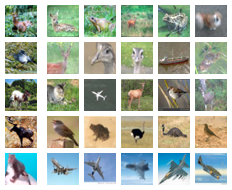
\includegraphics[width=0.28\linewidth]{figures/samples/refinenet128_cifar10_L10_step120000_5nearest.png}\label{fig:cifar10-nn}}\hspace{3mm}
     \subfloat[CelebA]{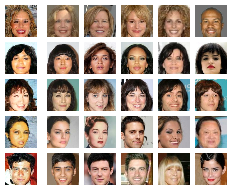
\includegraphics[width=0.28\linewidth]{figures/samples/refinenet128_celeb_a_L10_step30000_5nearest.png}\label{fig:celeba-nn}}
     \caption{$k=5$ nearest neighbours from the training data for 5 samples based on $l_2$-distance.}
     \label{fig:nn}
     \vspace{-3mm}
\end{figure}

\subsection{Inpainting}
We also performed inpainting as in \cite{ncsn-paper}, occluding the right half of the image and completing the image with annealed Langevin dynamics. The results are shown in \autoref{fig:inpainting}. As we can see, the models perform extremely well, especially in recovering the background for CIFAR-10 and the right half of the face for CelebA. Moreover, inpaintings for the same image are diverse, which showcases the generalisation capacity of the approach. Furthermore, one advantage of this method is that it is able to handle arbitrary occlusion shapes well (\autoref{fig:celeb_a_inpainting} in the Appendix). A nice addition would be to quantify the quality of results by measuring signal-to-noise ratio, but we leave this as future work.\vspace{-3mm}

\begin{figure}[h!]
  \centering
     \subfloat[MNIST]{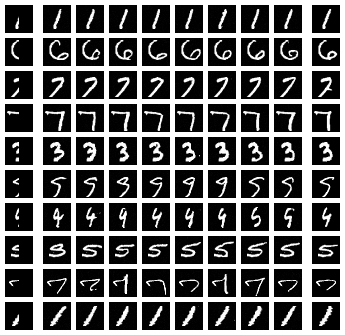
\includegraphics[width=0.311\linewidth]{figures/samples/refinenet64_mnist_L10_step200000_inpainting.png}\label{fig:mnist-inpainting}}\hspace{1mm}
     \subfloat[CIFAR-10]{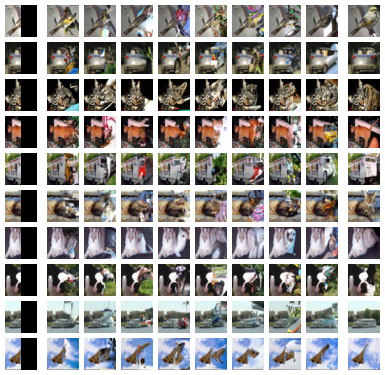
\includegraphics[width=0.311\linewidth]{figures/samples/refinenet128_cifar10_L10_step120000_inpainting.png}\label{fig:cifar10-inpainting}}\hspace{1mm}
     \subfloat[CelebA]{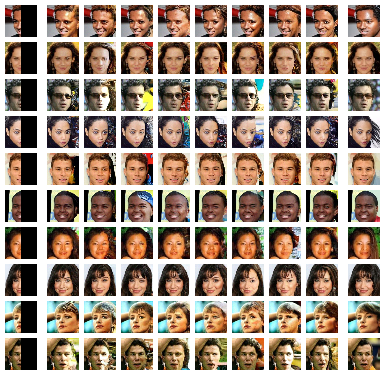
\includegraphics[width=0.311\linewidth]{figures/samples/refinenet128_celeb_a_L10_step30000_inpainting.png}\label{fig:celeba-inpainting}}
     \caption{Inpainting for occluded images from the training set. The occluded image is given in the leftmost column, and the true image in the rightmost column.}
     \label{fig:inpainting}
\end{figure}\vspace{-4mm}



\section{Additional experiments}
\label{sec:additional}
After successfully reproducing most of the experiments, we thought of some interesting extensions. Specifically, we investigated the choice of sampling hyperparameters $\epsilon$ and $T$, annealing schedule and network architecture, which we identified as important but unexplored in the original work. \vspace{-0.9mm}

\subsection{Sensitivity on sampling parameters}
The authors report the interval $\epsilon \in (5\cdot 10^{-6}, 5\cdot 10^{-5})$ and $T = 100$ as robust hyperparameters for sampling. Motivated by sensitivity to $\epsilon$ in the toy examples, we investigate these hyperparameters in more detail on real data from the CIFAR-10 dataset. We sampled with a smaller $\epsilon$ (\autoref{fig:1e-6eps}) and a larger $\epsilon$ (\autoref{fig:1e-1eps}), where the former yielded only noise since the step was not large enough to move away from the noisy initial point, and the latter resulted in samples being one-coloured because too large step size escaped allowed pixel values and was artificially clipped to the endpoints of pixel intervals. Similarly, a large $T$ results in smoother images (\autoref{fig:t-1000}), but with much fewer details, probably due to convergence to a local mode representing some kind of generic class image, and a small $T$ (\autoref{fig:t-10}) being mostly noise with only slightly distinguishable shapes. While the reasoning here is speculative, we here would like to emphasise the sensitivity to choice of $\epsilon$ and $T$, as already seen in the toy GMM experiment in \autoref{sec:repr-of-toy}. A suggested future work might concern different annealing strategies where $\epsilon$ or $T$ could be adjusted for different noise levels.\vspace{-2mm}

\begin{figure}[h!]
    \centering
    \subfloat[$\epsilon=10^{-6}, T=100$]{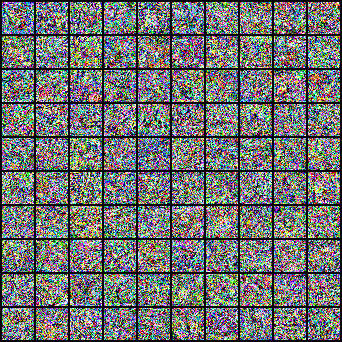
\includegraphics[width=0.24\linewidth]{figures/samples/samples_eps/1e-6.png}\label{fig:1e-6eps}}\hspace{1mm}
    \subfloat[$\epsilon=10^{-1}, T=100$]{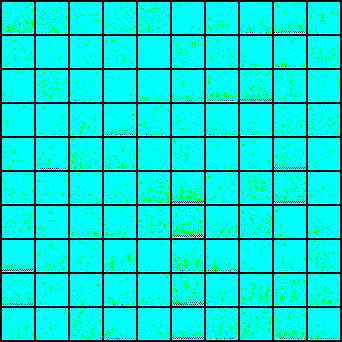
\includegraphics[width=0.24\linewidth]{figures/samples/samples_eps/1e-1.png}\label{fig:1e-1eps}}\hspace{1mm}
    \subfloat[$\epsilon=2\cdot 10^{-5}, T=10$]{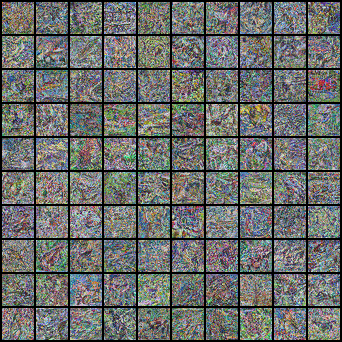
\includegraphics[width=0.24\linewidth]{figures/samples/samples_T/refinenet128_cifar10_L10_step120000_t10.png}\label{fig:t-10}}\hspace{1mm}
    \subfloat[$\epsilon=2\cdot 10^{-5}, T=10^3$]{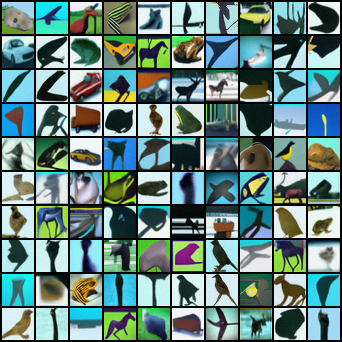
\includegraphics[width=0.24\linewidth]{figures/samples/samples_T/refinenet128_cifar10_L10_step120000_t1000.png}\label{fig:t-1000}}
     \caption{Samples from the best CIFAR-10 model with different values of $\epsilon$ and $T$.}
     \label{fig:varying-epsilon}
\end{figure}
% Considering that the step size of the annealed Langevin dynamic is proportional to the hyperparameter $\epsilon$, we can expect the behaviour observed in Figure \ref{fig:varying-epsilon}. If $\epsilon$ is too small, the image takes too small steps towards high density regions, and therefore never reaches them, remaining noisy. On the other hand, if the value of $\epsilon$ is too large, we speculate that the images converge to predominant modes that probably have large support.
 
\subsection{Linear annealing schedule}
We also train a model with linear annealing schedule instead of geometric on CIFAR-10 dataset. We hypothesise that geometric annealing might be too aggressive in the sense that most of noise values are low, which results in fine-tuning edges without capturing global features first. This is manifested in some samples being smooth, but not having a distinct shape of any reasonable object. From visual inspection of the results (\autoref{fig:linear}) we can see that intuition was correct, as these samples capture much more detail and complexity than with geometric annealing (\autoref{fig:cifar10-samp}). However, the images are visibly more noisy. We can explain this tendency using the inverse of the previous logic, namely that there are not enough noise levels in the low spectrum of values, thus precluding the sampling of sharper images. We believe some combination of these annealing schedules could solve this issue and result in very good samples, but also add to the complexity of the model.\vspace{-3mm}

\begin{figure}[h!]
    \centering
    \subfloat[50k iterations]{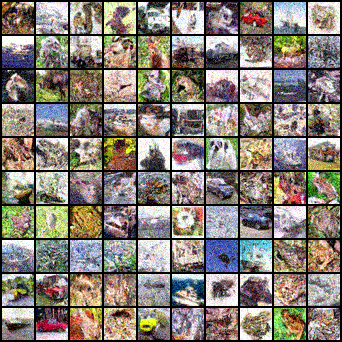
\includegraphics[width=0.24\linewidth]{figures/samples/linear/linear-50k.png}\label{fig:linear-50k}}\hspace{1mm}
    \subfloat[100k iterations]{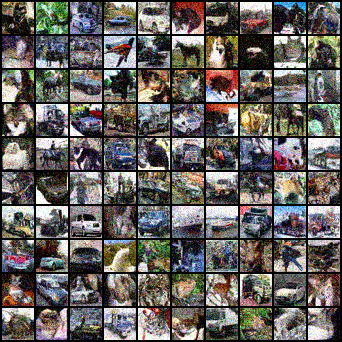
\includegraphics[width=0.24\linewidth]{figures/samples/linear/linear-100k.png}\label{fig:linear-100k}}\hspace{1mm}
    \subfloat[150k iterations]{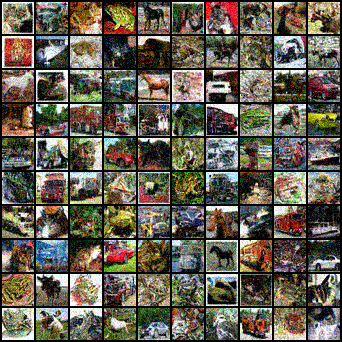
\includegraphics[width=0.24\linewidth]{figures/samples/linear/linear-150k.png}\label{fig:linear-150k}}\hspace{1mm}
    \subfloat[200k iterations]{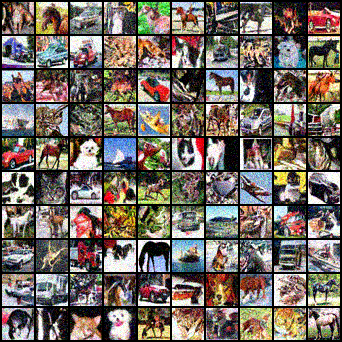
\includegraphics[width=0.24\linewidth]{figures/samples/linear/linear-200k.png}\label{fig:linear-200k}}
     \caption{Samples from model trained on CIFAR-10 with linear annealing schedule.}
     \label{fig:linear}
     \vspace{-3mm}
\end{figure}

\subsection{Different architecture of the score network}
The authors emphasise the choice of network architecture as important role and leave experimenting with different designs as future work. We address this by replacing the U-Net structure with the ResNet from the toy example in \autoref{sec:repr-of-toy} on CIFAR-10, but to avoid changing the architecture too much, we add conditional instance normalisation and dilated convolutions, as well as multiplying the number of filters by factor of 4 in each block to match the number of parameters in the RefineNet. Here we can only conclude that this simple architecture did not result in meaningful samples and that the choice of structure seems to be important. We believe the main reason for these subpar results is lack of skip connections as in U-Net type architectures. We also acknowledge that training hyperparameters would have to be tuned for this network to meaningfully compare the results. However, when taken in combination with the results from the main experiments in \autoref{sec:main-exp}, and assuming that our hypothesis -- that minor differences in RefineNet architecture between our implementation and the one from the original paper contribute to significantly worse performance in terms of FID score -- is correct, this would suggest that the method is perhaps overly reliant on architectural details. We suggest that more investigation is needed to determine exactly which aspects of the score network architecture are crucial for good performance.

\begin{figure}[H]
    \centering
    \subfloat[100k iterations]{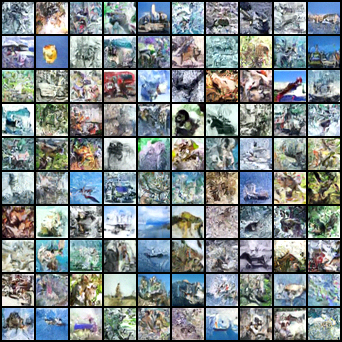
\includegraphics[width=0.31\linewidth]{figures/samples/resnet_100k.png}\label{fig:resnet-100k}}\hspace{1mm}
    \subfloat[150k iterations]{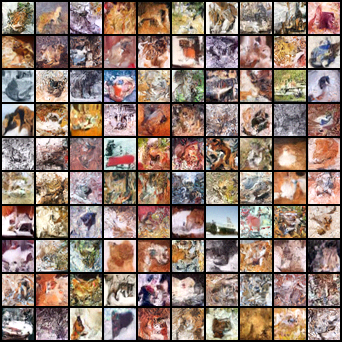
\includegraphics[width=0.31\linewidth]{figures/samples/resnet_150k.png}\label{fig:resnet-150k}}\hspace{1mm}
    \subfloat[200k iterations]{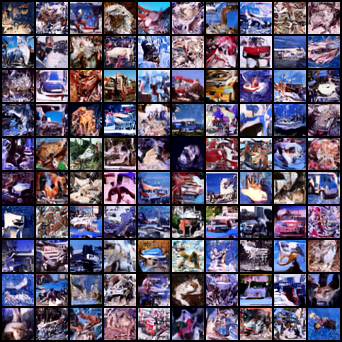
\includegraphics[width=0.31\linewidth]{figures/samples/resnet_200k.png}\label{fig:resnet-200k}}
     \caption{Samples from a ResNet model trained on CIFAR-10.}
     \label{fig:resnet}
\end{figure}

\section{Conclusions}
We can conclude that the main results from \cite{ncsn-paper} concerning image generation and inpainting are qualitatively reproducible and that the method indeed does yield visually good samples and inpainting results. However, we did not manage to obtain state-of-the-art Inception score on CIFAR-10 (nor comparable FID) as in \cite{ncsn-paper}, perhaps due to mentioned differences in the score network (which additional results show to be an important aspect of the method) or highly variable evaluation metric. When it comes to toy experiments used to investigate challenges and motivate assumptions of the proposed method, we report partial irreproducibility due to incorrectly reported noise levels for the annealed sampling from the given GMM. This observation led us to investigate the effect of different hyperparameters on sampling for CIFAR-10, which showed relatively high sensitivity to $\epsilon$ and $T$. We also experimented with a different architecture, and linear annealing schedule. While with the former we did not manage to generate reasonable samples (perhaps due to simplicity of the architecture), the latter yielded more detailed (but slightly more noisy) samples than the default geometric annealing, thus paving the path for future improvements. 






\small

\bibliographystyle{unsrtnat}
\bibliography{bibliography}

\clearpage
\section*{Appendix}

\vspace{5cm}

\begin{figure}[h!]
  \centering
     \subfloat[$\epsilon \in \{ 10^{-1},10^{-2},10^{-3},10^{-4},10^{-5},10^{-6} \}$.]{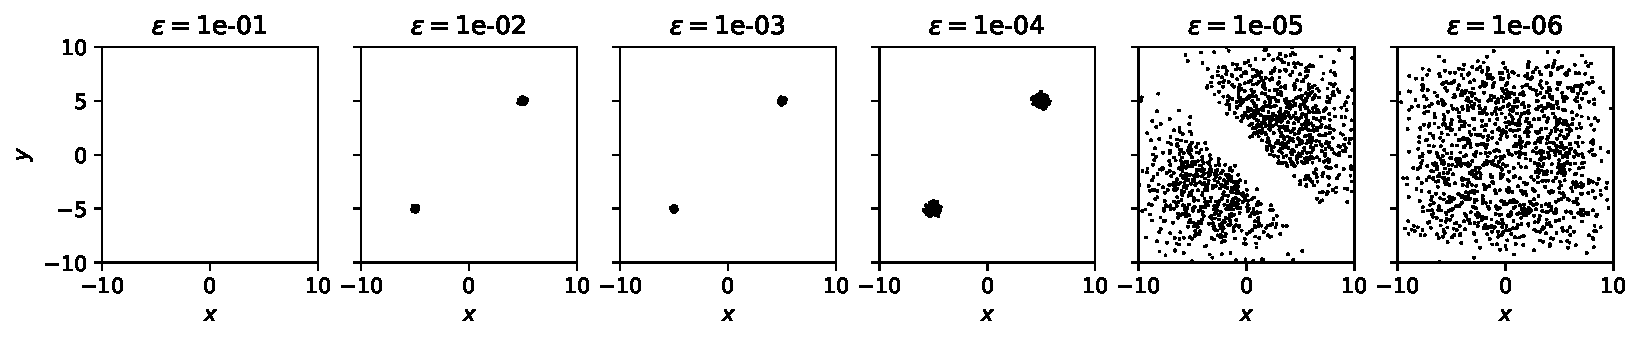
\includegraphics[width=\linewidth]{figures/toy/samples_eps_1.pdf}}\\
     \subfloat[$\epsilon \in \{ 10^{-4},8 \cdot 10^{-5},6 \cdot 10^{-5},4 \cdot 10^{-5},2 \cdot 10^{-5}, 10^{-5} \}$.]{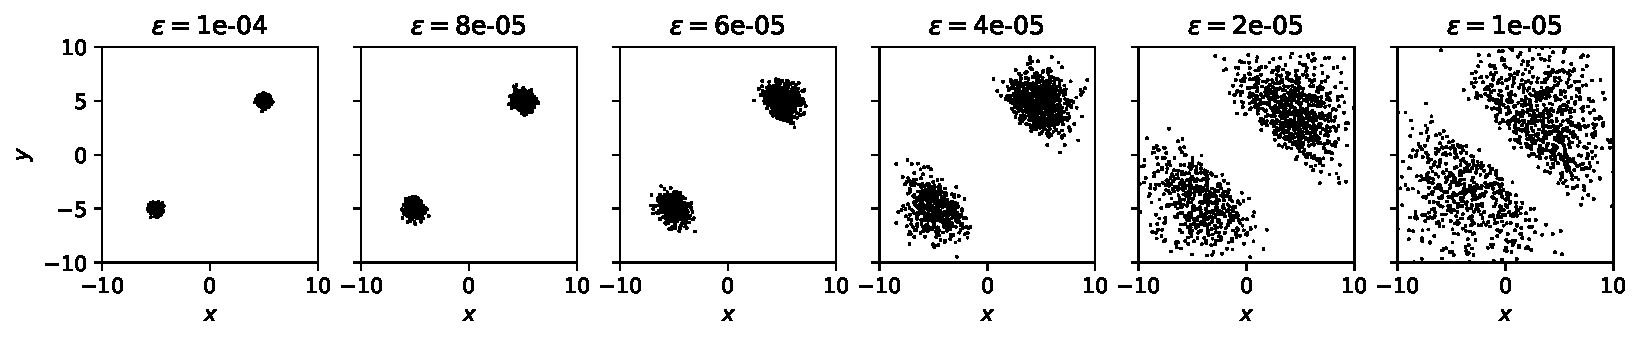
\includegraphics[width=\linewidth]{figures/toy/samples_eps_2.pdf}}
     \caption{Samples obtained with different values of $\epsilon$ for toy data with annealed Langevin dynamics. Even after expanding the search in the promising interval $\epsilon \in \{10^{-4}, 10^{-5}\}$, we did not find a value of $\epsilon$ yielding satisfying results.}
     \label{fig:eps}
\end{figure}


% \vspace{1cm}
\newpage


\begin{figure}[h!]
    \centering
    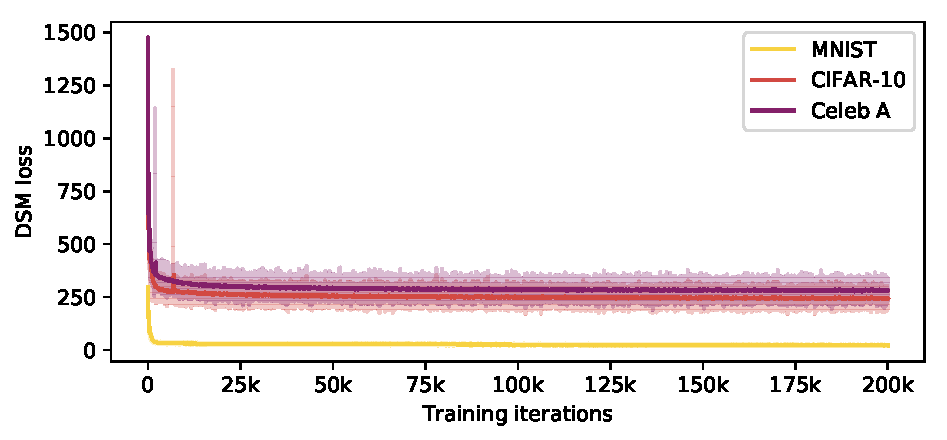
\includegraphics[width=0.90\linewidth]{figures/loss_real.pdf}
    \caption{Loss curves for training real model}
    \label{fig:losses}
\end{figure}

\vspace{0.8cm}

\begin{figure}[h!]
    \centering
    \subfloat[CIFAR10]{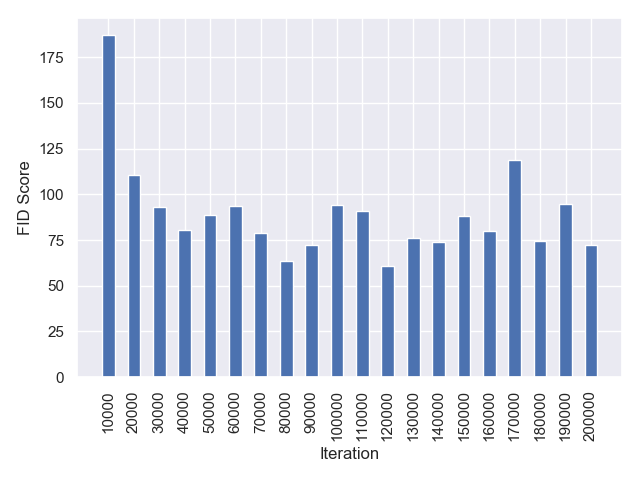
\includegraphics[width=0.47\linewidth]{figures/fid_plots/fid_score_cifar10.png}}
    \subfloat[CelebA]{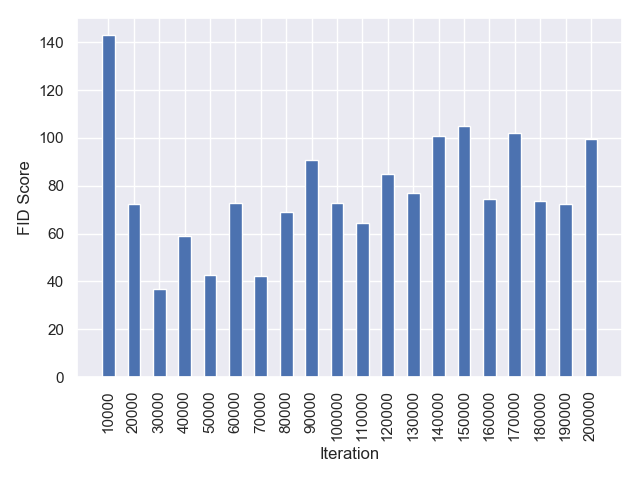
\includegraphics[width=0.47\linewidth]{figures/fid_plots/fid_score_celeb_a.png}}
    \caption{FID scores on 1000 samples for the model trained up to given iteration}
    \label{fig:fid}
\end{figure}

\vspace{1cm}

\begin{table}[h!]
    \centering
    \begin{tabular}{l c c c}
    \toprule
         & \multicolumn{3}{c}{Dataset} \\ \cmidrule{2-4}
         & MNIST & CIFAR-10 & CelebA \\ \midrule     
    Downloading data (required once) & 28.7s & 50.4s & 715.4s \\
    Training with RefineNet & 2.35it/sec & 1.73it/sec & 1.73it/sec \\
    Sampling (1 image) & 19s & 23s & 23s \\
    Sampling (100 images) & 112s & 158s & 158s \\
    Sampling (1000 images) & 910s & 1398s & 1398s \\ \bottomrule
    \end{tabular}
    \vspace{3mm}
    \caption{Time required for different components of the main experiment for each dataset. MNIST was run on a P100 GPU, while the other two datasets were run on a V100 GPU.}
    \label{tab:times}
\end{table}


\begin{figure}[h!]
    \centering
    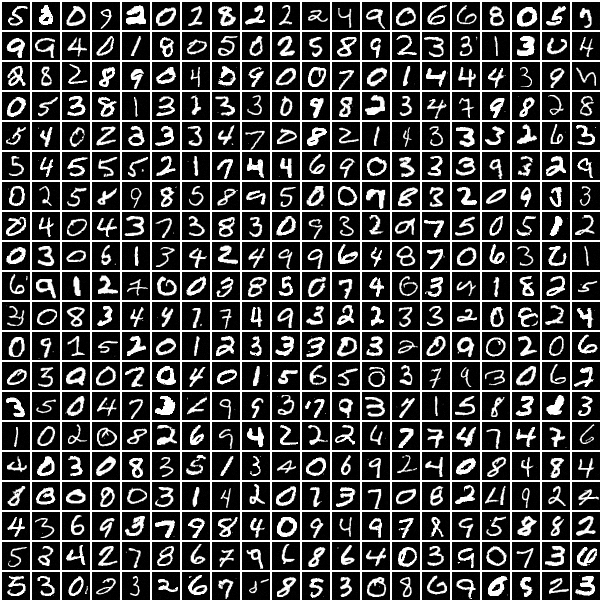
\includegraphics[width=\linewidth]{figures/samples/mnist_samples_large.png}
    \caption{Extended samples from MNIST}
    \label{fig:mnist-samples-large}
\end{figure}

\begin{figure}[h!]
    \centering
    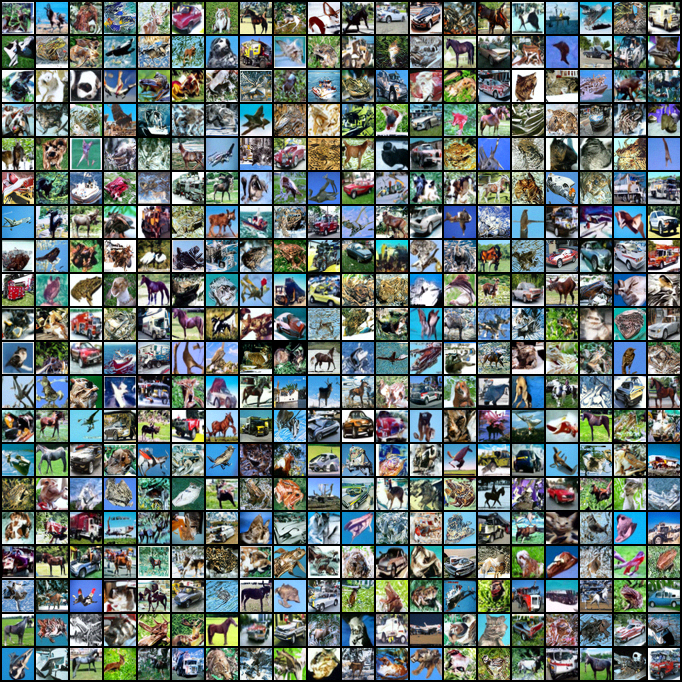
\includegraphics[width=\linewidth]{figures/samples/refinenet128_cifar10_L10_step120000_20x20.png}
    \caption{Extended samples from CIFAR10}
    \label{fig:cifar10-samples-large}
\end{figure}

\begin{figure}[h!]
    \centering
    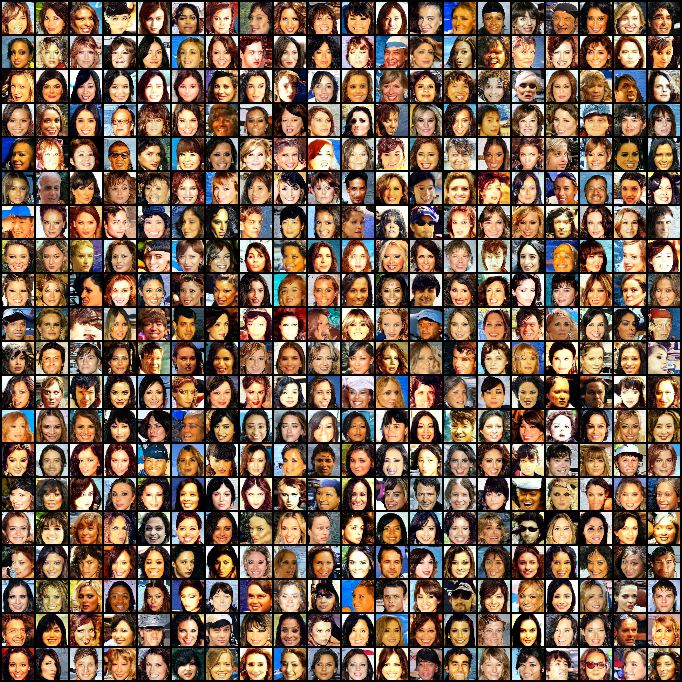
\includegraphics[width=\linewidth]{figures/samples/celeba_samples_large.png}
    \caption{Extended samples from CelebA}
    \label{fig:celeba-samples-large}
\end{figure}


\begin{figure}[h!]
  \centering
     \subfloat[MNIST]{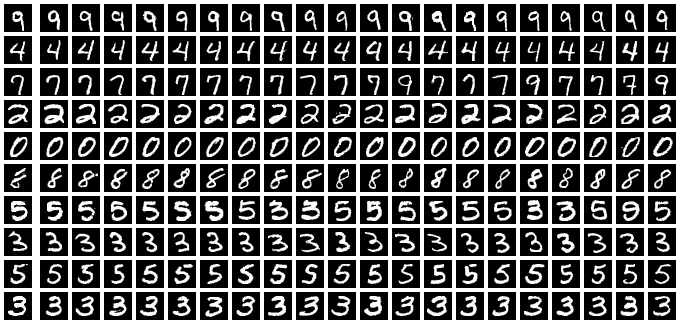
\includegraphics[width=0.91\linewidth]{figures/samples/refinenet64_mnist_L10_step200000_20nearest.png}\label{fig:mnist-nearest}}\\
     \subfloat[CIFAR-10]{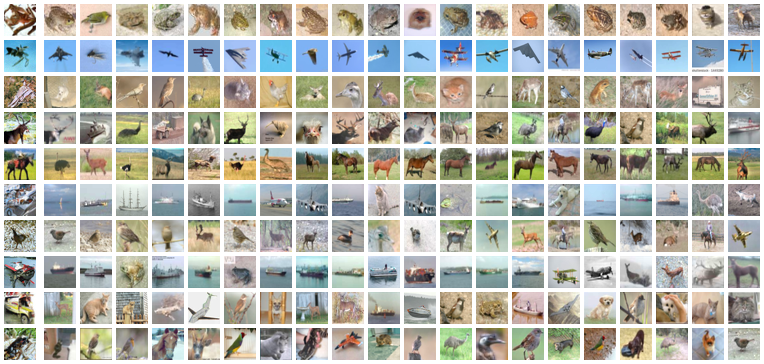
\includegraphics[width=0.9\linewidth]{figures/samples/refinenet128_cifar10_L10_step120000_20nearest.png}\label{fig:cifar10-nearest}}\\
     \subfloat[CelebA]{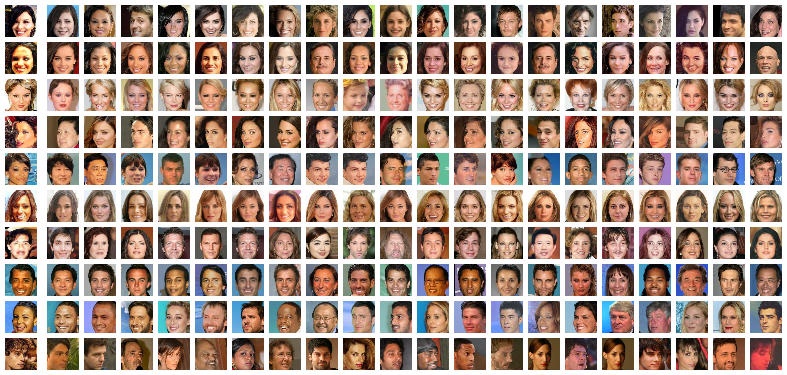
\includegraphics[width=0.9\linewidth]{figures/samples/refinenet128_celeb_a_L10_step30000_20nearest.png}\label{fig:celeba-nearest}}
     \caption{Samples (leftmost column) and their nearest neighbours from training set w.r.t. $l_2$ distance.}
     \label{fig:nn-large}
\end{figure}

\begin{figure}
    \centering
     \subfloat{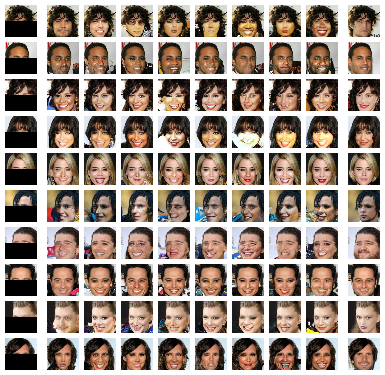
\includegraphics[width=0.75\linewidth]{figures/samples/refinenet128_celeb_a_L10_step30000_inpainting_occluded_down.png}\label{fig:celeb_a-inpaint_down}}\\
     \subfloat{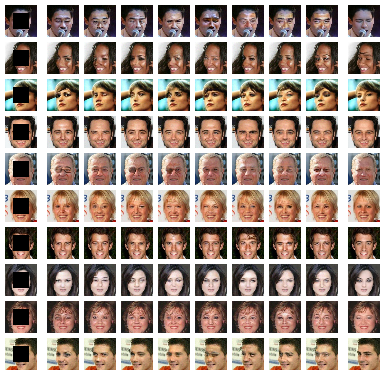
\includegraphics[width=0.75\linewidth]{figures/samples/other_occlusions/refinenet128_celeb_a_L10_step30000_inpainting_centered.png}\label{fig:celeb_a-inpaint_centered}}\\
     \caption{Recontruction with two more different patterns of occlusions on CelebA. Note that unlike the left-right occlusions shown in the main results, utilising face symmetry is not possible with these occlusions, once again proving the method has a good generative capacity.}
    \label{fig:celeb_a_inpainting}
\end{figure}

\end{document}
